\section{Planificación inicial}\label{sec:planif_inicial}
Como se ha mencionado anteriormente, se utiliza la metodología \textit{Scrum}
para la planificación y desarrollo del proyecto. En la figura \ref{fig:backlog}
se puede ver el \textit{backlog} de tareas que se planifican en el proyecto.

\begin{figure}[H]
	\centering
	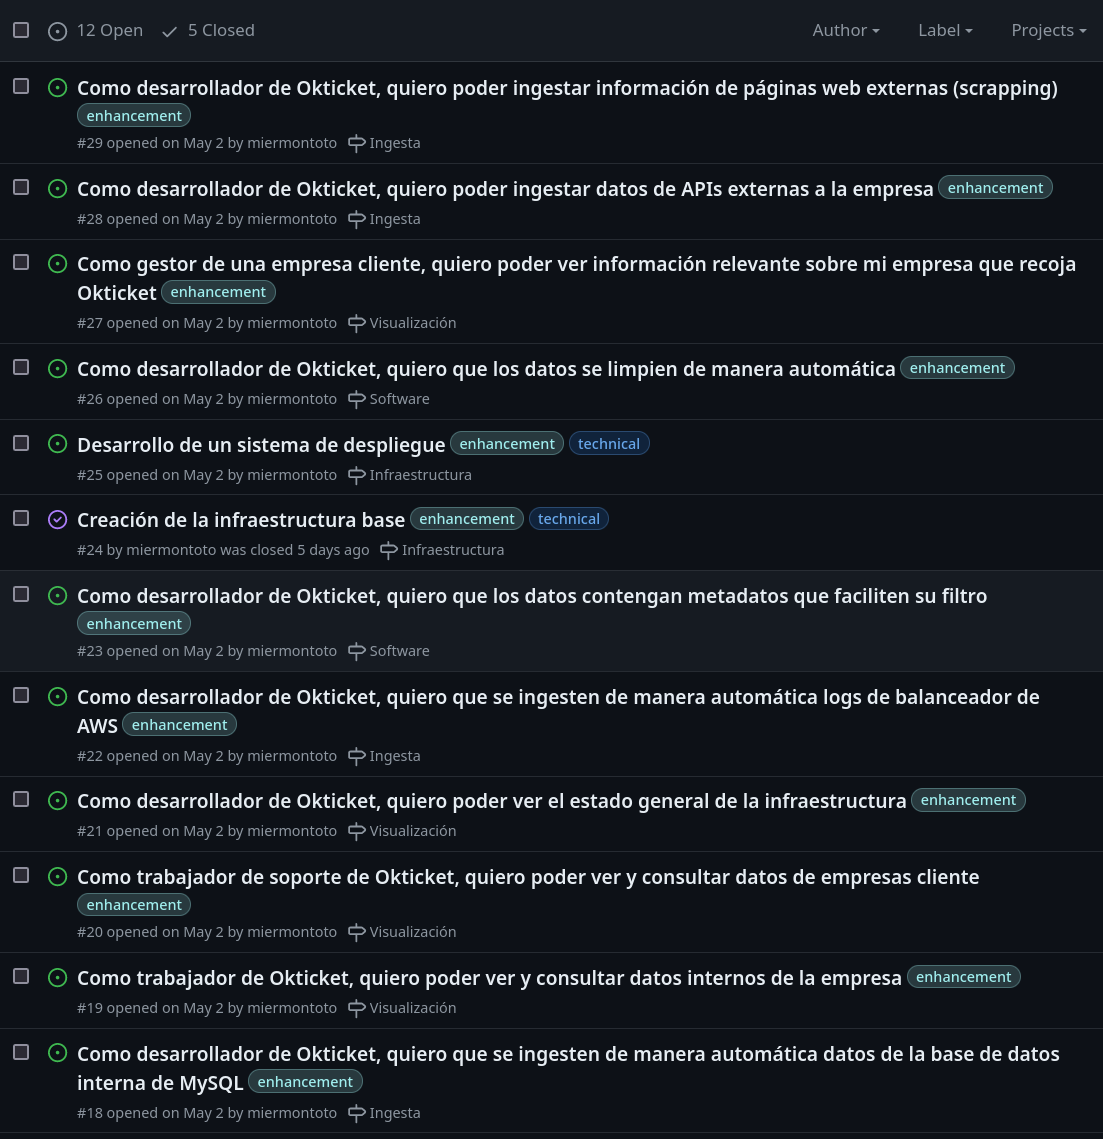
\includegraphics[width=\textwidth]{planif/backlog.png}
	\caption{Planificación inicial del proyecto}
	\label{fig:backlog}
\end{figure}

Las historias de usuario anteriores se clasifican y categorizan según su
prioridad y tamaño, haciendo uso de la estrategia de tallas de camiseta como
mencionado anteriormente. En el tablero \textit{Kanban}
(ver figura \ref{fig:kanban}) se puede ver en todo momento el estado de las HU,
su progreso y sus características. El listado inicial (ordenado según su prioridad)
es el siguiente:

\begin{table}[H]
	\centering
	\begin{tabular}{|p{0.7\linewidth}|c|c|}
		\hline
		\textbf{Nombre} & \textbf{Prioridad} & \textbf{Tamaño} \\
		\hline
		\hline
		Creación de la infraestructura base (técnica) & P0\cellcolor{red!50} & L\cellcolor{orange!50} \\
		\hline
		Como desarrollador de Okticket, quiero que la arquitectura se despliegue y orqueste de manera automática & P0\cellcolor{red!50} & XL\cellcolor{red!50} \\
		\hline
		Como desarrollador de Okticket, quiero que se ingesten de manera automática datos de la base de datos interna de MongoDB & P0\cellcolor{red!50} & M\cellcolor{yellow!50} \\
		\hline
		Como desarrollador de Okticket, quiero que se ingesten de manera automática datos de la base de datos interna de MySQL & P0\cellcolor{red!50} & M\cellcolor{yellow!50} \\
		\hline
		Como desarrollador de Okticket, quiero que los datos se limpien de manera automática & P0\cellcolor{red!50} & M\cellcolor{yellow!50} \\
		\hline
		Como trabajador de Okticket, quiero poder ver y consultar datos internos de la empresa & P1\cellcolor{orange!50} & L\cellcolor{orange!50} \\
		\hline
		Como desarrollador de Okticket, quiero que se ingesten de manera automática logs de balanceador de AWS & P1\cellcolor{orange!50} & S\cellcolor{green!25} \\
		\hline
		Como desarrollador de Okticket, quiero poder ver el estado general de la infraestructura & P1\cellcolor{orange!50} & L\cellcolor{orange!50} \\
		\hline
		Como desarrollador de Okticket, quiero que los datos contengan metadatos que faciliten su filtrado o búsqueda & P2\cellcolor{yellow!50} & S\cellcolor{green!25} \\
		\hline
		Como trabajador de Okticket, quiero poder ver y consultar datos de empresas cliente & P2\cellcolor{yellow!50} & M\cellcolor{yellow!50} \\
		\hline
		Como gestor de una empresa cliente, quiero poder ver información relevante sobre mi empresa que recoja Okticket & P2\cellcolor{yellow!50} & L\cellcolor{orange!50} \\
		\hline
		Como desarrollador de Okticket, quiero poder ingestar datos de APIs externas a la empresa & P2\cellcolor{yellow!50} & L\cellcolor{orange!50} \\
		\hline
		Como desarrollador de Okticket, quiero poder ingestar información de páginas web externas (\textit{scraping}) & P2\cellcolor{yellow!50} & XL\cellcolor{red!50} \\
		\hline
	\end{tabular}
	\caption{Historias de usuario iniciales}
	\label{tab:initial_tasks}
\end{table}

Siguiendo la tabla anterior, se pueden planear los \textit{sprints} y
asignar las tareas a cada uno de ellos.
